\documentclass[tikz,border=0pt,11pt]{standalone}
\usepackage[T1]{fontenc}
\usepackage[utf8]{inputenc}
\usepackage{lmodern,amsmath,amssymb}
\usepackage[swedish]{babel}
\usetikzlibrary{arrows.meta,calc,positioning,decorations.pathmorphing,decorations.pathreplacing,patterns,shadings}
\definecolor{navy}{HTML}{102F40}
\definecolor{teal}{HTML}{147D78}
\definecolor{lightteal}{HTML}{E6F1ED}
\definecolor{gold}{HTML}{B88B3B}
\definecolor{palegold}{HTML}{F7EEDB}
\definecolor{rust}{HTML}{B6533B}
\definecolor{palerust}{HTML}{FAEAE4}
\definecolor{paper}{HTML}{F7F5EE}
\definecolor{muted}{HTML}{5B6D72}
\definecolor{line}{HTML}{D6DED8}
\renewcommand{\familydefault}{\sfdefault}
\newcommand{\atom}[5]{\shade[ball color=#3!70] (#1,#2) circle (#5);\node[text=white,font=\bfseries\small] at (#1,#2){#4};}
\newcommand{\water}[3]{\begin{scope}[shift={(#1,#2)},scale=#3]\draw[navy!45,line width=2pt] (-.3,.22)--(0,0)--(.3,.22);\atom{0}{0}{rust}{O}{.22}\atom{-.3}{.22}{teal}{H}{.15}\atom{.3}{.22}{teal}{H}{.15}\end{scope}}
\newcommand{\panel}[4]{\filldraw[fill=white,draw=line,rounded corners=5pt] (#1,#2) rectangle ++(#3,#4);}
\newcommand{\note}[4]{\node[txt,text width=#3cm] at (#1,#2){#4};}
\tikzset{txt/.style={anchor=north west,align=left,text=navy,font=\small},
 head/.style={anchor=west,text=navy,font=\bfseries\large},
 label/.style={align=center,text=navy,font=\small},
 smalllabel/.style={align=center,text=muted,font=\footnotesize},
 arrow/.style={-{Latex[length=2.5mm,width=1.8mm]},line width=1.2pt,draw=teal},
 goldarrow/.style={-{Latex[length=2.5mm]},line width=1.2pt,draw=gold},
 rustarrow/.style={-{Latex[length=2.5mm]},line width=1.2pt,draw=rust},
 dashedarrow/.style={arrow,dashed},
 badge/.style={fill=lightteal,rounded corners=3pt,text=teal,font=\bfseries\small,inner sep=5pt}}
\begin{document}
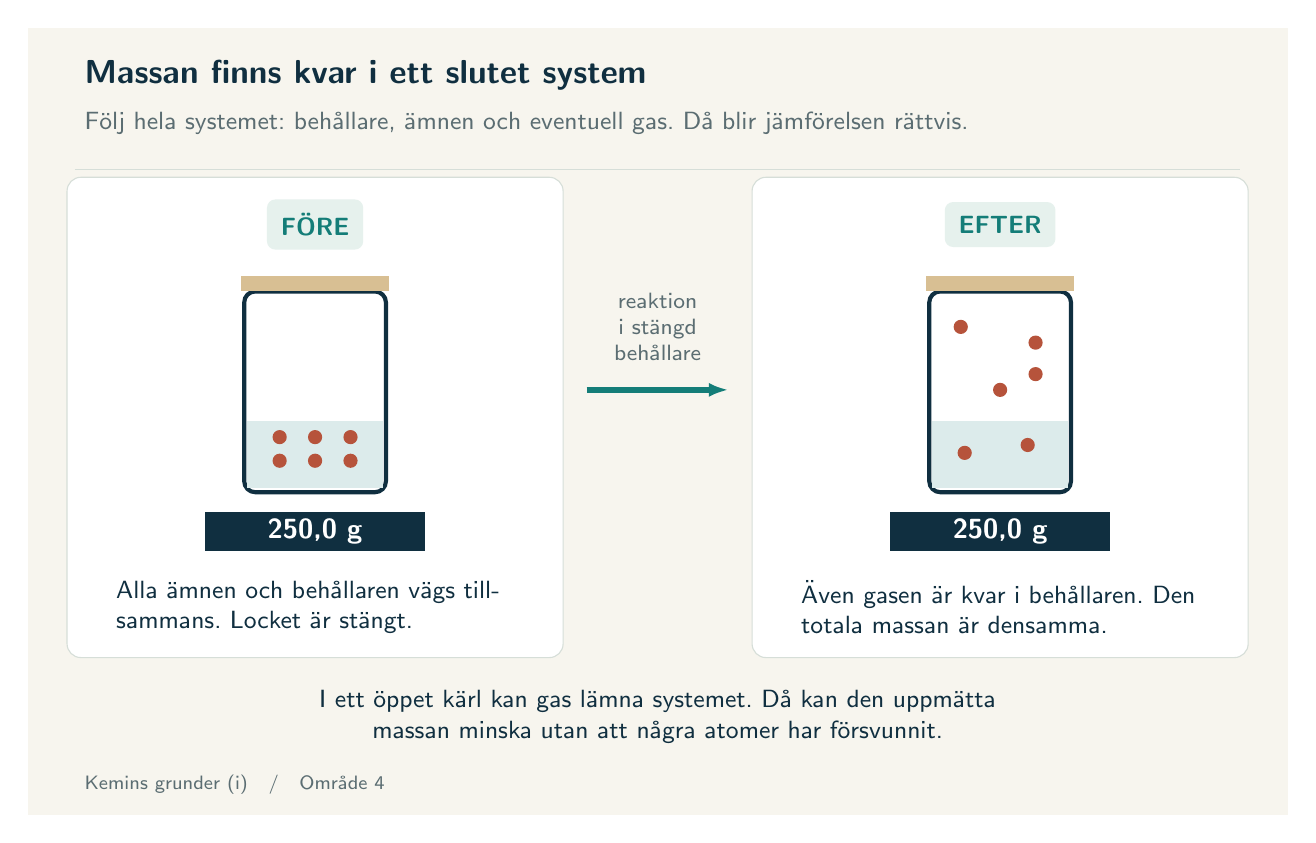
\begin{tikzpicture}[x=1cm,y=1cm]
\path[use as bounding box] (0,0) rectangle (16,10);
\fill[paper] (0,0) rectangle (16,10);
\node[head] at (.6,9.4){Massan finns kvar i ett slutet system};
\note{.6}{9.05}{14.8}{\textcolor{muted}{Följ hela systemet: behållare, ämnen och eventuell gas. Då blir jämförelsen rättvis.}}
\draw[line] (.6,8.2)--(15.4,8.2);

\panel{.5}{2}{6.3}{6.1}\panel{9.2}{2}{6.3}{6.1}
\node[badge] at (3.65,7.5){FÖRE};\node[badge] at (12.35,7.5){EFTER};
\foreach \cx in {3.65,12.35}{\draw[navy,line width=1.5pt,rounded corners=4pt] (\cx-.9,4.1) rectangle(\cx+.9,6.65);\fill[gold!55] (\cx-.94,6.65) rectangle(\cx+.94,6.85);\fill[teal!15] (\cx-.86,4.15) rectangle(\cx+.86,5);\fill[navy] (\cx-1.4,3.35) rectangle(\cx+1.4,3.85);\node[text=white,font=\bfseries] at (\cx,3.6){250,0 g};}
\foreach \x/\y in {3.2/4.5,3.65/4.5,4.1/4.5,3.2/4.8,3.65/4.8,4.1/4.8}{\fill[rust] (\x,\y) circle(.09);}
\foreach \x/\y in {11.9/4.6,12.35/5.4,12.8/6,11.85/6.2,12.7/4.7,12.8/5.6}{\fill[rust] (\x,\y) circle(.09);}
\draw[arrow,line width=2pt] (7.1,5.4)--(8.9,5.4);\node[smalllabel,text width=2cm] at (8,6.2){reaktion i stängd behållare};
\note{1}{3.1}{5.3}{Alla ämnen och behållaren vägs tillsammans. Locket är stängt.}
\note{9.7}{3.1}{5.3}{Även gasen är kvar i behållaren. Den totala massan är densamma.}
\node[label,text width=14cm] at (8,1.25){I ett öppet kärl kan gas lämna systemet. Då kan den uppmätta massan minska utan att några atomer har försvunnit.};\node[anchor=west,text=muted,font=\scriptsize] at (.6,.38){Kemins grunder (i)\quad /\quad Område 4};

\end{tikzpicture}\end{document}
